\documentclass{beamer}
\usetheme{tokitex}
\usepackage{graphics}
\usepackage{multirow}
\usepackage{tabto}
\usepackage[english,bahasa]{babel}
\newtranslation[to=bahasa]{Section}{Bagian}
\newtranslation[to=bahasa]{Subsection}{Subbagian}

\usepackage{listings}
\usepackage{color}

\definecolor{dkgreen}{rgb}{0,0.6,0}
\definecolor{gray}{rgb}{0.5,0.5,0.5}
\definecolor{mauve}{rgb}{0.58,0,0.82}

\lstset{frame=tb,
  aboveskip=0mm,
  belowskip=0mm,
  language=pascal,
  showstringspaces=false,
  columns=flexible,
  basicstyle={\small\ttfamily},
  numbers=none,
  numberstyle=\tiny\color{gray},
  keywordstyle=\color{blue},
  commentstyle=\color{dkgreen},
  stringstyle=\color{mauve},
  breaklines=true,
  breakatwhitespace=true,
  tabsize=2
}

\title{Analisis Kompleksitas}
\author{Tim Olimpiade Komputer Indonesia}

\begin{document}

\begin{frame}
\titlepage
\end{frame}

\begin{frame}
\frametitle{Pendahuluan}
Melalui dokumen ini, kalian akan:
\begin{itemize}
	\item Memahami konsep analisis kompleksitas.
	\item Mampu menganalisis kompleksitas untuk memperkirakan \textit{runtime} eksekusi program.
\end{itemize}
\end{frame}

\section{Pengenalan Analisis Algoritma}
\frame{\sectionpage}

\begin{frame}
\frametitle{Analisis Algoritma}
\begin{itemize}
	\item Diberikan dua algoritma untuk menyelesaikan permasalahan yang sama. Algoritma mana yang lebih cepat?
	\item Pengukuran seberapa cepatnya suatu algoritma biasa dinyatakan dalam kompleksitas waktu.
	\item Kompleksitas waktu: banyaknya komputasi yang perlu dilakukan dari awal eksekusi sampai berakhirnya algoritma. 
\end{itemize}
\end{frame}

\begin{frame}
\frametitle{Contoh Soal: Membajak Sawah}
Deskripsi:
\begin{itemize}
	\item Pak Dengklek memiliki $N$ bibit tanaman yang akan ia semai di sawahnya.
	\item Untuk itu, ia akan membajak sawahnya supaya sawahnya bisa memuat $N$ tanaman.
	\item Sawah yang akan dibajak harus memiliki bentuk persegi panjang, tersusun atas $R$ baris dan $C$ kolom petak-petak. Setiap petak bisa memuat maksimal sebuah tanaman.
	\item Tentukan nilai $R$ dan $C$ supaya semua petak yang ada ditanami tanaman!
	\item Jika ada lebih dari satu kemungkinan jawaban, minimalkan selisih R dengan C.
	\item Jika masih ada lebih dari satu kemungkinan jawaban, cetak yang mana saja.
\end{itemize}
\end{frame}

\begin{frame}
\frametitle{Contoh Soal: Membajak Sawah (lanj.)}
Batasan:
\begin{itemize}
	\item $1 \le N \le 10^9$.
\end{itemize}

\hfill

Format Masukan:
\begin{itemize}
	\item Sebuah baris berisi bilangan bulat, yaitu $N$.
\end{itemize}

\hfill

Format Keluaran:
\begin{itemize}
	\item Sebuah baris berisi dua bilangan bulat, yaitu $R$ dan $C$.
\end{itemize}

\end{frame}

\begin{frame}
\frametitle{Contoh Soal: Membajak Sawah (lanj.)}

\begin{block}{Contoh Masukan}
35
\end{block}

\hfill

\begin{block}{Contoh Keluaran}
7 5
\end{block}

\end{frame}

\begin{frame}
\frametitle{Solusi 1: Coba Semua Kemungkinan}
\begin{itemize}
	\item Untuk setiap $R$ dan $C$ yang mungkin, coba hitung apakah $R \times C$ sama dengan $N$.
	\item Jika ya, cari yang selisih $|R-C|$ minimal.
	\item Cukup mencoba untuk $1 \le R \le N$ dan $1 \le C \le N$.
\end{itemize}
\end{frame}

\begin{frame}[fragile]
\frametitle{Solusi 1: Coba Semua Kemungkinan (lanj.)}
Bagian implementasi:
\begin{lstlisting}
readln(N);
R := 1;
C := N;
for i := 1 to N begin
  for j := 1 to N do begin
    if (i*j = N) then begin
      if (abs(R-C) > abs(i-j)) then begin
        R := i;
        C := j;	
      end;
    end;
  end;
end
writeln(R, ' ', C);
\end{lstlisting}
\end{frame}

\begin{frame}[fragile]
\frametitle{Solusi 1: Coba Semua Kemungkinan (lanj.)}
\begin{itemize}
	\item Misalkan untuk $N = 100$, secara kasar diperlukan $100 \times 100$ komputasi untuk mencari nilai $R$ dan $C$ yang tepat.
	\item Jadi secara umum bisa diperkirakan bahwa untuk suatu nilai $N$, diperlukan $N^2$ komputasi.
	\item Solusi ini dikatakan memiliki kompleksitas waktu sebesar $O(N^2)$ (dibaca "O-N-kuadrat").
	\item Pertanyaan: apakah solusi ini cukup cepat? Bagaimana jika $N = 10^9$?
\end{itemize}
\end{frame}

\begin{frame}
\frametitle{Cerita Sampingan: Meramal Waktu Eksekusi}
\begin{itemize}
	\item Terdapat sebuah perkiraan kasar bahwa komputer mampu melakukan 100 juta ($10^8$) komputasi dalam $1$ detik.
	\item Tentu saja, perkiraan ini masih sangat kasar. Waktu untuk melakukan $10^8$ operasi penjumlahan tidak sama dengan waktu untuk melakukan $10^8$ operasi modulo.
	\item Jenis bahasa pemrograman juga mempengaruhi waktu eksekusi algoritma, misalnya bahasa C cenderung lebih cepat daripada Java.
	\item Bagaimanapun juga, konvensi ini umum digunakan pada dunia pemrograman kompetitif dan sesuai untuk bahasa Pascal, C, dan C++.
\end{itemize}
\end{frame}

\begin{frame}
\frametitle{Solusi 1: Terlalu lambat!}
\begin{itemize}
	\item Untuk $N$ yang bisa mencapai $10^9$, diperlukan sekitar $10^{18}/10^8 = 10^{10}$ detik.
	\item Waktu tersebut setara dengan sekitar 317 tahun!
	\item Adakah solusi lebih efisien?
\end{itemize}
\end{frame}

\begin{frame}
\frametitle{Solusi 2: Coba Semua Kemungkinan $R$}
\begin{itemize}
	\item Tidak perlu memeriksa semua $R$ dan $C$, cukup coba saja semua kemungkinan $R$ untuk $1 \le R \le N$. 
	\item Jika untuk suatu nilai $R$, diketahui $N$ habis dibagi $R$, maka $C$ dipastikan ada, yaitu $N/R$.
\end{itemize}
\end{frame}

\begin{frame}[fragile]
\frametitle{Solusi 2: Coba Semua Kemungkinan $R$ (lanj.)}
Bagian implementasi:
\begin{lstlisting}
readln(N);
R := 1;
C := N;
for i := 1 to N begin
  if (N mod i = 0) then begin
    j := N div i;
    if (abs(R-C) > abs(i-j)) then begin
      R := i;
      C := j;  
    end;
  end;
end;
writeln(R, ' ', C);
\end{lstlisting}
\end{frame}

\begin{frame}[fragile]
\frametitle{Solusi 2: Coba Semua Kemungkinan $R$ (lanj.)}
\begin{itemize}
	\item Solusi ini bekerja dengan lebih cepat.
	\item Untuk suatu nilai $N$, kasarnya cukup dilakukan $N$ komputasi untuk mencari nilai $R$ dan $C$ yang tepat.
	\item Solusi ini dikatakan memiliki kompleksitas waktu sebesar $O(N)$.
	\item Untuk $N = 10^9$, diperlukan sekitar 10 detik eksekusi algoritma.
\end{itemize}
\end{frame}

\begin{frame}[fragile]
\frametitle{Solusi 3: Batasi $R$ sampai $\sqrt{N}$}
\begin{itemize}
	\item Persoalan ini sebenarnya meminta kita memfaktorkan $N$, supaya dua bilangan hasil faktorisasi sedekat mungkin.
	\item Untuk memeriksa seluruh faktor bilangan, cukup batasi sampai $\sqrt{N}$ saja. 
	\item Contoh: untuk $N = 100$, faktorisasi yang mungkin adalah:
	\begin{itemize}
		\item $1 \times 100$
		\item $2 \times 50$
		\item $4 \times 25$
		\item $5 \times 20$
		\item $10 \times 10$
		\item $20 \times 5$
		\item $25 \times 4$
		\item $...$ (faktorisasi selanjutnya hanya mengulang yang sudah ada)
	\end{itemize}
\end{itemize}
\end{frame}

\begin{frame}[fragile]
\frametitle{Solusi 3: Batasi $R$ sampai $\sqrt{N}$ (lanj.)}
Bagian implementasi:
\begin{lstlisting}
readln(N);
R := 1;
C := N;

i := 1;
while (i*i <= N) do begin
  if (N mod i = 0) then begin
    j := N div i;
    if (abs(R-C) > abs(i-j)) then begin
      R := i;
      C := j;
    end;
  end;
  i := i + 1;
end
writeln(R, ' ', C);
\end{lstlisting}
\end{frame}

\begin{frame}[fragile]
\frametitle{Solusi 3: Batasi $R$ sampai $\sqrt{N}$ (lanj.)}
\begin{itemize}
	\item Kompleksitas solusi menjadi hanya $O(\sqrt{N})$.
	\item Untuk $N = 10^9$, hanya diperlukan sekitar 32.000 komputasi, jauh di bawah 100 juta.
	\item Solusi ini bekerja dengan cepat bahkan untuk $N$ yang besar.
\end{itemize}
\end{frame}

\begin{frame}
\frametitle{Ulasan Contoh Soal}
\begin{itemize}
	\item Untuk menyelesaikan suatu permasalahan, bisa jadi ada beberapa solusi, masing-masing dengan kompleksitasnya tersendiri.
	\item Dari ketiga solusi yang telah dijelaskan, solusi ketiga sudah pasti paling diharapkan untuk bisa menyelesaikan permasalahan.
	\item Untuk mengukur seberapa efisien suatu algoritma, bisa digunakan notasi Big-Oh untuk kompleksitas waktu.
\end{itemize}
\end{frame}

\begin{frame}
\frametitle{Notasi Big-Oh}
\begin{itemize}
	\item Biasa digunakan pada ilmu komputer untuk menyatakan pertumbuhan nilai suatu fungsi terhadap ukuran masukan yang diberikan.
	\item Dalam kasus ini, fungsi yang dimaksud adalah fungsi banyaknya komputasi yang diperlukan jika diberikan suatu ukuran masukan.
	\item Kita tidak akan menggali terlalu dalam tentang hal-hal matematis di balik notasi Big-Oh ini, hanya kulit luarnya saja.
\end{itemize}
\end{frame}

\begin{frame}
\frametitle{Aturan Sederhana Notasi Big-Oh}
\begin{enumerate}
	\item Konstanta bisa diabaikan.
	
	Contoh: $O(3N^2)$ bisa ditulis $O(N^2)$ saja.
	
	Alasan: kita hanya tertarik dengan \textbf{pertumbuhan fungsinya}, bukan nilai fungsi sebenarnya.
	
	\hfill
	
	\item Cukup ambil suku yang mendominasi.
	
	Contoh: $O(N^3 + N^2)$ bisa ditulis $O(N^3)$ saja.
	
	Alasan: untuk $N$ yang besar, suku $N^3$ akan jauh lebih besar daripada suku $N^2$, sehingga $N^2$ menjadi tidak signifikan.
	
\end{enumerate}
\end{frame}

\begin{frame}
\frametitle{Kelompok Kompleksitas}
Biasanya kompleksitas dikelompokkan menurut kelasnya sebagai berikut:
\begin{itemize}
	\item \textit{Constant}: $O(1)$
	
	Komputasi yang dilakukan tidak bergantung pada besarnya input. Contoh: program untuk mencari nilai harga mutlak suatu angka.
	
	\item \textit{Logarithmic}: $O(\log{N})$
	
	Komputasi yang dilakukan proporsional terhadap nilai logaritma dari input. 
	
\end{itemize}
\end{frame}

\begin{frame}
\frametitle{Kelompok Kompleksitas (lanj.)}
\begin{itemize}
	\item \textit{Linear}: $O(N)$
	
	Komputasi yang dilakukan proporsional secara linier terhadap input.
	
	\item \textit{Polynomial}: $O(\sqrt{N})$, $O(N^2)$, $O(N^3), ...$
	 
	Komputasi yang dilakukan proporsional secara polinomial terhadap input.
	
	\item \textit{Exponential}: $O(N!)$, $O(2^N)$, $O(N^N), ...$
		 
	Komputasi yang dilakukan proporsional secara eksponensial terhadap input. Biasanya dihindari karena terlalu lambat.
		
\end{itemize}
\end{frame}

\begin{frame}
\frametitle{Kelompok Kompleksitas (lanj.)}
\begin{figure}
	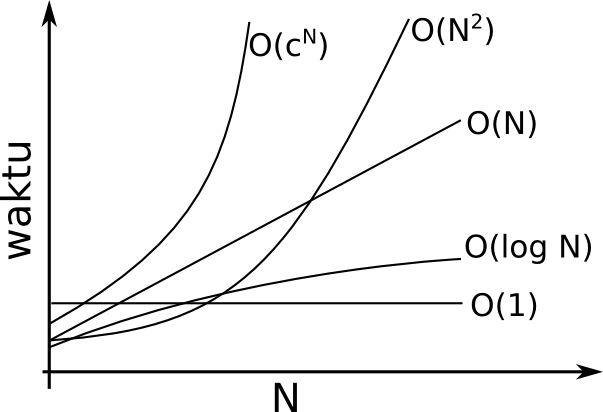
\includegraphics[width=8cm]{asset/grafik.png}
\end{figure}
\end{frame}

\section{Menghitung Kompleksitas}
\frame{\sectionpage}

\begin{frame}
\frametitle{Menghitung Kompleksitas}
\begin{itemize}
	\item Wajib dilakukan sebelum mengimplementasikan suatu algoritma.
	\item Tujuannya untuk memperkirakan apakah solusi ini cukup efisien untuk menyelesaikan persoalan yang ada.
	\item Dengan sedikit latihan, Anda dapat menghitung kompleksitas dari algoritma sederhana.
\end{itemize}
\end{frame}

\begin{frame}[fragile]
\frametitle{Contoh 1: Soal}
Hitung kompleksitas waktu potongan program berikut:

\hfill

\begin{lstlisting}
total := 0;
for i := 1 to N do begin
  for j := 1 to N do begin
    total := total + 1;
  end;
end;
\end{lstlisting}
\end{frame}

\begin{frame}
\frametitle{Contoh 1: Jawaban}
\begin{itemize}
	\item Sederhana, jawabannya adalah $O(N^2)$.
\end{itemize}
\end{frame}

\begin{frame}[fragile]
\frametitle{Contoh 2: Soal}
Hitung kompleksitas waktu potongan program berikut:

\hfill

\begin{lstlisting}
total := 0;
for i := 1 to N do begin
  for j := i to N do begin
    total := total + 1;
  end;
end;
\end{lstlisting}
\end{frame}

\begin{frame}
\frametitle{Contoh 2: Jawaban}
\begin{itemize}
	\item Banyaknya operasi "total := total + 1" yang dilakukan adalah $N + (N-1) + (N-2) + ... + 2 + 1 = \frac{N(N+1)}{2}$.
	\item Kompleksitasnya $O \left( \frac{N(N+1)}{2} \right)$, tetapi cukup ditulis $O(N^2)$ saja.
\end{itemize}
\end{frame}

\begin{frame}[fragile]
\frametitle{Contoh 3: Soal}
Hitung kompleksitas waktu potongan program berikut:

\hfill

\begin{lstlisting}
total := 0;
for i := 1 to N do begin
  for j := 1 to M do begin
    total := total + 1;
  end;
end;
\end{lstlisting}
\end{frame}

\begin{frame}
\frametitle{Contoh 3: Jawaban}
\begin{itemize}
	\item Kali ini terdapat dua variabel pada input, yaitu $N$ dan $M$.
	\item Kompleksitasnya adalah $O(NM)$.
\end{itemize}
\end{frame}

\begin{frame}[fragile]
\frametitle{Contoh 4: Soal}
Hitung kompleksitas waktu potongan program berikut:

\hfill

\begin{lstlisting}
val := N;
while (val > 0) do begin
  val := val div 3;
end;
\end{lstlisting}
\end{frame}

\begin{frame}
\frametitle{Contoh 4: Jawaban}
\begin{itemize}
	\item Banyaknya operasi yang dilaksanakan setara dengan panjang dari barisan $\frac{N}{3}, \frac{N}{9}, \frac{N}{27}, ..., 1$.
	\item Panjang dari barisan tersebut sebenarnya adalah logaritma basis 3 dari $N$, atau bisa dituliskan kompleksitasnya $O(\log_3{N})$.
	\item Namun sebenarnya $\log_3{N} = \frac{\log{N}}{\log{3}}$.
	\item Berhubung $\log{3}$ adalah konstanta, jadi cukup ditulis $O(\log{N})$ saja.
\end{itemize}
\end{frame}

\begin{frame}[fragile]
\frametitle{Contoh 5: Soal}
Hitung kompleksitas waktu potongan program berikut:

\hfill

\begin{lstlisting}
counter := 1;
while (counter*counter < N) do begin
  counter := counter + 1;
end;
\end{lstlisting}
\end{frame}

\begin{frame}
\frametitle{Contoh 5: Jawaban}
\begin{itemize}
	\item Nilai variabel $counter$ akan terus bertambah, hingga kuadratnya lebih dari $N$.
	\item Misalkan jika $N = 81$, maka $counter$ akan berhenti setelah nilainya melebihi $9$.
	\item Kompleksitas sebenarnya adalah $O(\sqrt{N})$.
\end{itemize}
\end{frame}

\begin{frame}
\frametitle{Penutup}
\begin{itemize}
	\item Pelajari lebih lanjut tentang perhitungan kompleksitas melalui latihan yang diberikan.
	\item Terdapat notasi lainnya yang tidak kita bahas di sini, seperti Big-Theta ($\Theta$), Big-Omega ($\Omega$), Little-Oh (o), dan sebagainya. Silakan Anda pelajari jika tertarik untuk mengetahui lebih lanjut.
\end{itemize}
\end{frame}

\end{document}